\documentclass[10pt]{article}

\setlength{\textheight}{25.7cm}
\setlength{\textwidth}{16cm}
\setlength{\unitlength}{1mm}
\setlength{\topskip}{2.5truecm}
\topmargin 260mm \advance \topmargin -\textheight 
\divide \topmargin by 2 \advance \topmargin -1in 
\headheight 0pt \headsep 0pt \leftmargin 210mm \advance
\leftmargin -\textwidth 
\divide \leftmargin by 2 \advance \leftmargin -1in 
\oddsidemargin \leftmargin \evensidemargin \leftmargin
\parindent=0pt

\frenchspacing

\usepackage{microtype}
\usepackage{array}
\usepackage{amsmath}
\usepackage{graphicx}

\usepackage[dutch]{babel}

\usepackage{listings}
% Er zijn talloze parameters ...
\lstset{language=C++, showstringspaces=false, basicstyle=\small,
  numbers=left, numberstyle=\tiny, numberfirstline=false, breaklines=true,
  stepnumber=1, tabsize=8, 
  commentstyle=\ttfamily, identifierstyle=\ttfamily,
  stringstyle=\itshape}

\title{Verslag derde programmeeropdracht}

\author{Alex Keizer \& L\'{e}on van Velzen}

\begin{document}

\maketitle
\section{Uitleg programma}

Life is origineel bedacht door John Conway. De ``wereld" bestaat uit een 2-dimensionaal vlak van cellen, die levend of dood zijn. Een volgende generatie wordt d.m.v.\ twee simpele regels bepaald:
\begin{itemize}
\item Een levende cel overleeft alleen als het precies 2 of 3 levende buren heeft
\item Een dode cel met 3 levende buren komt weer tot leven
\end{itemize}
Met buren worden de acht direct of diagonaal aanliggende cellen bedoeld. In de theorie is de wereld oneindig groot, wij hebben ons beperkt tot $1000 \times 1000$. Deze simpele regels zorgen voor vrij complex gedrag, zie bijvoorbeeld de glidergun\cite{glidergun} en de acorn besproken in Paragraaf \ref{sec:acorn}

De gebruiker ziet slechts een $80 \times 25$ deel van de wereld tegelijk, de zogeheten ``view". Hij kan zijn view bewegen m.b.v.\ de \verb+wasd+ toetsen. Verder is er onder de view een menu te vinden waarmee het programma bestuurd wordt.

\section{Acorn}\label{sec:acorn}

Waar de glidergun als het ware een geweer is dat continu gliders produceert, is de `acorn'\cite{acorn} het beste als een explosief te beschrijven. Hij begint simpel, de start configuratie bestaat uit slechts 7 cellen (zie Figuur \ref{fig:gen0}). 

\begin{figure}[!ht]
\begin{center}
{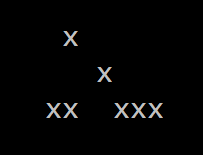
\includegraphics[scale=0.5]{gen0.png}}
\caption{De start configuratie van de acorn}\label{fig:gen0}
\end{center}
\end{figure}

In het begin breidt de vorm langzaam uit. Rond generatie 130 zien we dat de actie vooral naar links gebeurd, rechts zien we eigenlijk alleen 2 stabiele $2\times2$ blokken en een `blinker' (zie Figuur \ref{fig:gen130}). Deze vormen zien we rond generatie 300 nogsteeds, er zijn zelfs nog meer stabiele vormen verschenen (zie Figuur \ref{fig:gen300}).

\begin{figure}[!ht]
\begin{center}

\begin{minipage}{.5\textwidth}
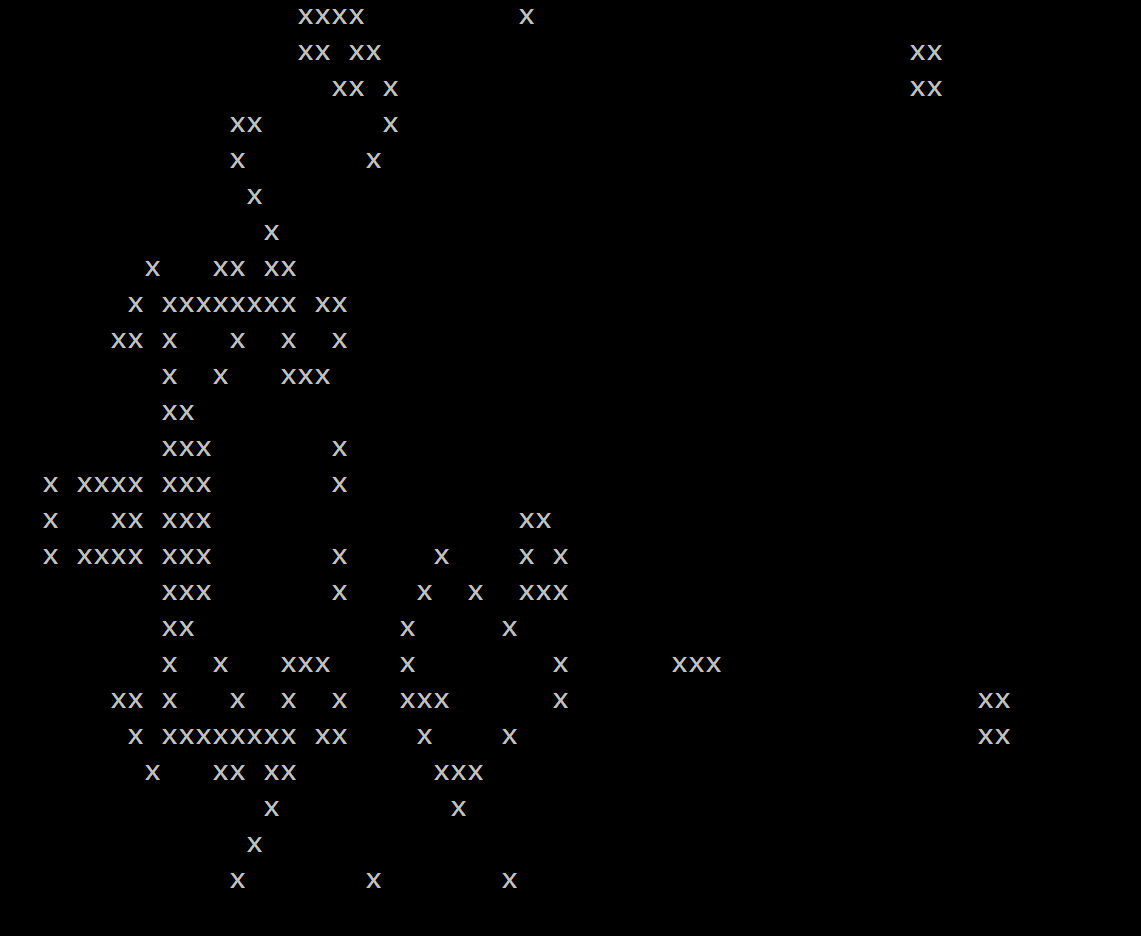
\includegraphics[width=0.75\linewidth]{gen130.png}
\caption{Generatie 130}\label{fig:gen130}
\end{minipage}%
\begin{minipage}{.5\textwidth}
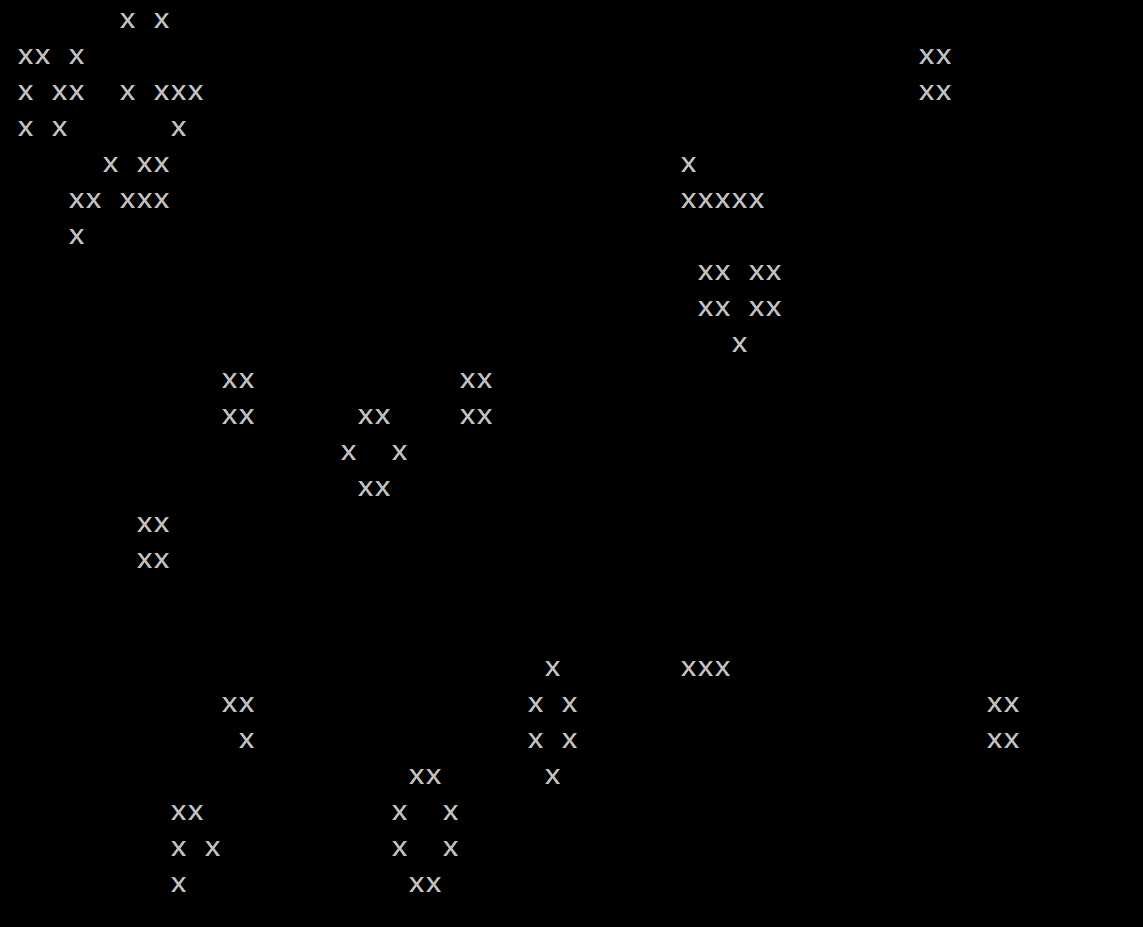
\includegraphics[width=0.75\linewidth]{gen300.png}
\caption{Generatie 300}\label{fig:gen300}
\end{minipage}

\end{center}
\end{figure}

Op dit punt zijn de interessante elementen helaas niet meer in de grootte van de view te zien, uiteindelijk zal de acorn in generatie 5206 zijn volgroeid tot een stabiel patroon (zie Figuur \ref{fig:final}.

\begin{figure}[!ht]
\begin{center}
{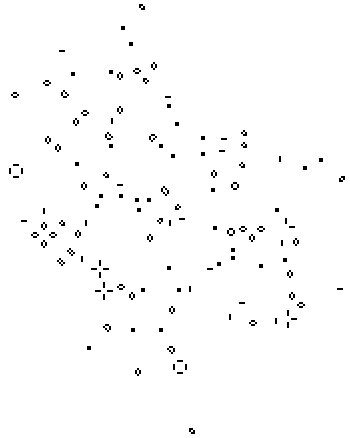
\includegraphics[scale=0.5]{Acorn_final.png}}
\caption{Generatie 5206, de stabiele staat \cite{acorn}}\label{fig:final}
\end{center}
\end{figure}

\newpage

\section{Tijd}

Tijd in uren besteed per week:

\begin{center}
\begin{tabular}{ |c|c|c| }
\hline
Week & Alex Keizer & L\'{e}on van Velzen \\
42 & 1 & 2,5 \\
43 & 0 & 2 \\
44 & 1 & 1 \\
45 & 5 & 0,5 \\ 
\hline
Totaal & 7 & 6 \\
\hline
\end{tabular}
\end{center}

Laatste wijziging op 10/11/2017

\begin{thebibliography}{9}
    \bibitem{glidergun} Gosper glider gun. Geraadpleegd op 9/11/2017, \\
van \verb+http://www.conwaylife.com/w/index.php?title=Gosper_glider_gun+

	\bibitem{acorn} Acorn. Geraadpleegd op 9/11/2017, 
van \verb+http://www.conwaylife.com/wiki/Acorn+
\end{thebibliography}

\section{Code}

\lstinputlisting{keizervanvelzen3.cpp}

\end{document}
